\graphicspath{ {./images/9_Repeatability} }
\newpage

\section{Repeatability (optional)}
For sample IDs that appear more than once in the dataset (e.g., \textsf{pool} or \textsf{VisuCon}), the repeatability of analyte relative abundances can be visualized. 
The repeatability for multiple sample IDs can be assessed by creating separate tabs using the \menu{Add a tab +} button in the top-right corner of the box.

In a tab, select the sample ID for which to visualize the repeatability.
Optionally, you toggle the option to visualize the repeatability per plate number.
Then click on \menu{Assess repeatability}.
An interactive bar plot is generated displaying the relative abundances of all analytes.
Error bars represent the [mean $\pm$ standard deviation (SD)] of each analyte.
The dots plotted over the bars indicate the relative standard deviations ($\text{RSD} = \text{SD} \times 100\%$).

\begin{center}
	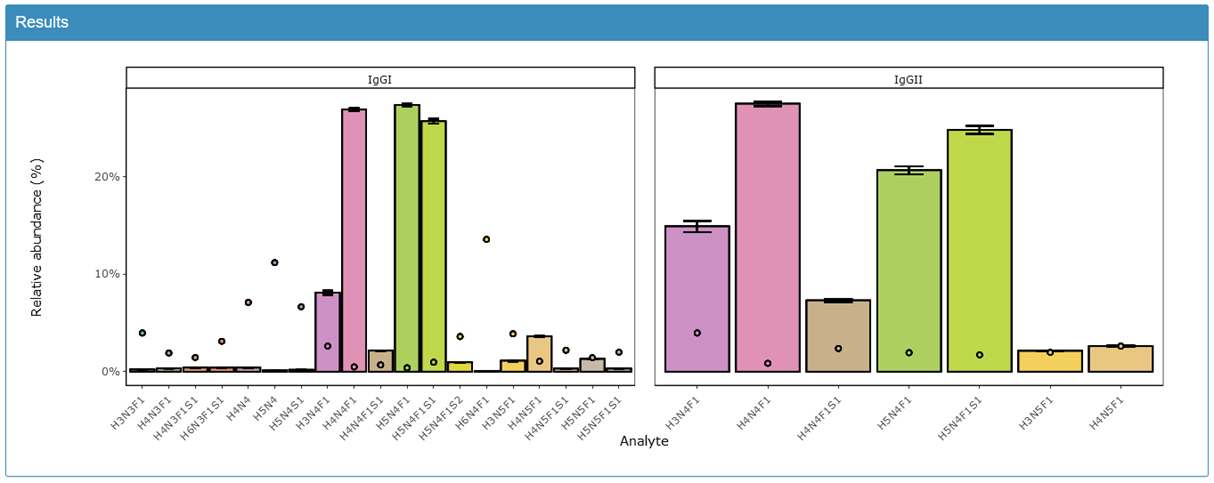
\includegraphics[scale=0.5]{repeatability.png}
\end{center}

When assessing the repeatability per plate, a table is presented showing median intra-plate variations, calculated as the median of the analyte RSDs on a plate.
At the bottom of the table, ther inter-plate variation is displayed, calculated as the mean of the intra-plate variations.

\begin{center}
	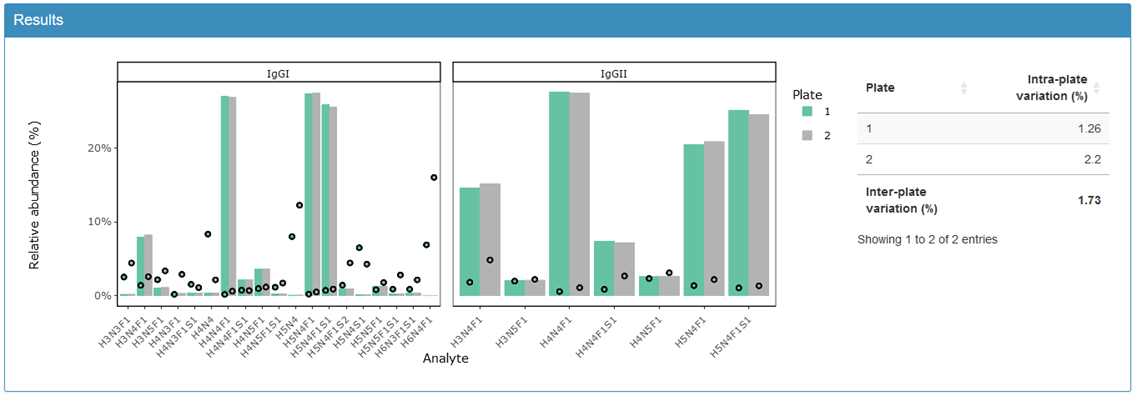
\includegraphics[scale=0.54]{repeatability_perplate.png}
\end{center}